\documentclass[11pt,letterpaper]{article}

% ===================== PACKAGES =====================
\usepackage[utf8]{inputenc}
\usepackage[english]{babel}
\usepackage[T1]{fontenc}
\usepackage[margin=2.5cm]{geometry}
\usepackage{amsmath,amssymb}
\usepackage{graphicx}
\usepackage{booktabs}
\usepackage{array}
\usepackage{xcolor}
\usepackage{siunitx}
\usepackage{hyperref}
\usepackage{enumitem}
\usepackage{caption}
\usepackage{fancyhdr}
\usepackage{tcolorbox}
\usepackage{circuitikz}
\ctikzset{bipoles/length=0.8cm}
\usepackage{float}
\tcbuselibrary{skins,breakable}

\hypersetup{
    colorlinks=true,
    linkcolor=blue!50!black,
    citecolor=blue!50!black,
    urlcolor=blue!50!black
}

\sisetup{output-decimal-marker={.}, group-separator={,}}

\pagestyle{fancy}
\fancyhf{}
\fancyhead[L]{Series RLC with Analog PID Control -- Project Logbook}
\fancyhead[R]{\thepage}
\renewcommand{\headrulewidth}{0.4pt}

\newtcolorbox{pending}{colback=yellow!8,colframe=orange!60!black,arc=1mm,breakable,title={PENDING}}

% ===================== DOCUMENT METADATA =====================
\title{\textbf{Overshoot Elimination in a Series RLC Circuit via Analog PID Control} \\[4pt]
\large Electronic Engineering Technical Documentation}
\author{Project Logbook}
\date{Version 0.2 --- \today}

\begin{document}

\maketitle

\begin{abstract}
\noindent This document describes the design, classical control analysis, and SPICE simulation of an
analog PID controller applied to a series RLC circuit, with the goal of eliminating the step-response
overshoot inherent to its underdamped open-loop dynamics. This is the first of two related projects; the
second applies the same PID design methodology to a buck converter (repository \texttt{BUCK\_1} covers an
earlier, IC-based adjustable buck design, not the PID-controlled version). Documented as an honest
engineering logbook: every result is marked as \textbf{calculated}, \textbf{simulated}, or
\textbf{pending} --- never filled in with invented placeholder data. The plant is fixed and its open-loop
overshoot confirmed both analytically (52.7\%) and in SPICE (52.68\%). The PID gains are derived via
pole placement ($K_p\approx27.87$, $K_i\approx455{,}905$, $K_d\approx3.114\times10^{-4}$) and the op-amp
compensator topology is defined. \textbf{Still open}: the specific R/C component values realizing those
gains, the full closed-loop schematic, and its SPICE validation --- explicitly marked \textbf{PENDING}.
\end{abstract}

\tableofcontents
\newpage

% ======================================================================
\section{Project Objective}

Design and validate an analog PID controller, implemented with operational amplifiers, that closes the
loop around a series RLC circuit and eliminates the overshoot present in its open-loop step response,
using classical control design methods (transfer function derivation, root locus / pole placement).
This project establishes the PID design methodology later applied to a discrete, analog-PID-controlled
buck converter (a separate, subsequent project).

% ======================================================================
\section{Plant: Series RLC Circuit}

\subsection{Design criteria}

Component values were not assigned; they were chosen to satisfy two criteria: (1) clearly underdamped
($\zeta$ well below 1) so the open-loop overshoot is unambiguous, and (2) a natural frequency practical
for breadboard construction and standard lab equipment (function generator + oscilloscope), avoiding
both breadboard-parasitic-dominated frequencies (too high) and impractically long observation times (too
low).

\begin{table}[H]
\centering
\caption{Design targets and resulting component values}
\begin{tabular}{@{}p{5cm}p{6cm}p{3.5cm}@{}}
\toprule
\textbf{Parameter} & \textbf{Value} & \textbf{Source} \\
\midrule
Target natural frequency, $f_0$ & \SI{5}{\kilo\hertz} & Defined by design \\
Target damping ratio, $\zeta$ & 0.2 (underdamped, $\approx$\SI{53}{\percent} overshoot target) & Defined by design \\
Capacitance, $C$ & \SI{100}{\nano\farad} & Defined by design (standard value) \\
Inductance, $L$ & \SI{10.13}{\milli\henry} & \textbf{Calculated}, Sec.~2.2 \\
Resistance, $R$ & \SI{127.32}{\ohm} & \textbf{Calculated}, Sec.~2.2 \\
\bottomrule
\end{tabular}
\end{table}

\subsection{Component value derivation}

With $\omega_n = 2\pi f_0 = 2\pi(5000) \approx \SI{31416}{rad/s}$, and the standard series-RLC relations:

\begin{tcolorbox}[colback=blue!5,colframe=blue!40!black,arc=1mm]
\begin{align}
L &= \frac{1}{\omega_n^2 C} \\
R &= 2\zeta\sqrt{L/C}
\end{align}
\end{tcolorbox}

\begin{align}
L &= \frac{1}{(31416)^2 (100\times10^{-9})} = \SI{10.13}{\milli\henry} \\
R &= 2(0.2)\sqrt{\frac{10.13\times10^{-3}}{100\times10^{-9}}} = \SI{127.32}{\ohm}
\end{align}

% ======================================================================
\section{Open-Loop Transfer Function}

With the capacitor voltage $V_C$ as the output and the source voltage $V_{in}$ as the input, the
standard second-order series-RLC transfer function is:

\begin{tcolorbox}[colback=blue!5,colframe=blue!40!black,arc=1mm]
\begin{equation}
\frac{V_C(s)}{V_{in}(s)} = \frac{1/LC}{s^2 + \dfrac{R}{L}s + \dfrac{1}{LC}} = \frac{\omega_n^2}{s^2+2\zeta\omega_n s+\omega_n^2}
\end{equation}
\end{tcolorbox}

with $\omega_n = 1/\sqrt{LC}$ and $\zeta = \frac{R}{2}\sqrt{C/L}$, confirming the values imposed by design
in Section~2.

\subsection{Predicted open-loop overshoot}

For an underdamped second-order system, the standard closed-form percent overshoot for a step input is:

\begin{equation}
\%OS = \exp\left(\frac{-\pi\zeta}{\sqrt{1-\zeta^2}}\right)\times 100
\end{equation}

With $\zeta=0.2$: $\%OS = \exp\left(\dfrac{-\pi(0.2)}{\sqrt{1-0.04}}\right)\times100 \approx \boxed{52.7\%}$.

This confirms the plant has substantial, clearly-visible open-loop overshoot -- a real problem for the
PID controller (Section~4) to solve, not a marginal one.

\subsection{SPICE confirmation}

\textbf{Simulated.} The circuit was built directly in LTspice (series $R$-$L$-$C$, driven by a
\SI{1}{\volt} step via a \texttt{PULSE} source, $V_C$ probed at the $L$-$C$ junction, \texttt{.tran 2m}).
The peak and final values were extracted numerically from the \texttt{.raw} binary file (not read
visually from the plot):

\begin{center}
\begin{tabular}{@{}ll@{}}
\toprule
Peak $V_C$ & \SI{1.52679}{\volt}, at $t=\SI{102.28}{\micro\second}$ \\
Final (settled) $V_C$ & \SI{1.00000}{\volt} \\
Overshoot & $(1.52679-1)/1 \times 100 = \boxed{52.68\%}$ \\
\bottomrule
\end{tabular}
\end{center}

This matches the analytical prediction (52.7\%) to within 0.02 percentage points, validating both the
transfer-function derivation and its SPICE implementation before any control is added.

% ======================================================================
\section{PID Controller Design}

\subsection{Parallel vs.\ series PID form}

Two classical structures exist for a PID compensator:

\begin{align}
\text{Parallel (ideal):} \quad & C(s) = K_p + \frac{K_i}{s} + K_d s \\
\text{Series (interacting):} \quad & C(s) = K_c\left(1+\frac{1}{T_i s}\right)(1+T_d s)
\end{align}

The series form is what results naturally from cascading a PI stage into a PD stage (fewer op-amps), but
its effective gains interact: expanding it gives $K_p = K_c(1+T_d/T_i)$, $K_i=K_c/T_i$, $K_d=K_cT_d$ --
changing $T_i$ also moves the effective $K_p$. \textbf{The parallel form was chosen} for this design: each
gain ($K_p$, $K_i$, $K_d$) is independently tunable, which maps directly onto the pole-placement method
used below (Section~4.3) and is more straightforward to justify/defend gain-by-gain.

\subsection{Why the closed-loop system is third order}

The plant $G(s)$ (Section~3) is second order (two energy-storage elements, $L$ and $C$). The controller
contributes exactly one additional pole, at $s=0$, from the integral term alone -- the $P$ and $D$ terms
add no poles. The full derivation, step by step:

\textbf{Step 1 -- combine $C(s)$ into a single fraction} (common denominator $s$):
\begin{equation}
C(s) = K_p + \frac{K_i}{s} + K_d s = \frac{K_p s}{s} + \frac{K_i}{s} + \frac{K_d s^2}{s} = \frac{K_d s^2 + K_p s + K_i}{s}
\end{equation}

\textbf{Step 2 -- multiply $C(s)G(s)$:}
\begin{equation}
C(s)G(s) = \frac{K_d s^2 + K_p s + K_i}{s}\cdot\frac{\omega_n^2}{s^2+2\zeta\omega_n s+\omega_n^2}
= \frac{\omega_n^2\left(K_d s^2+K_p s+K_i\right)}{s\left(s^2+2\zeta\omega_n s+\omega_n^2\right)}
\end{equation}

\textbf{Step 3 -- the characteristic equation is $1+C(s)G(s)=0$.} Clearing the denominator (multiplying
through by it):
\begin{equation}
s\left(s^2+2\zeta\omega_n s+\omega_n^2\right) + \omega_n^2\left(K_d s^2 + K_p s + K_i\right) = 0
\end{equation}

\textbf{Step 4 -- expand each product separately.} First term:
\begin{equation}
s\left(s^2+2\zeta\omega_n s+\omega_n^2\right) = s^3 + 2\zeta\omega_n s^2 + \omega_n^2 s
\end{equation}
Second term:
\begin{equation}
\omega_n^2\left(K_d s^2+K_p s+K_i\right) = \omega_n^2 K_d s^2 + \omega_n^2 K_p s + \omega_n^2 K_i
\end{equation}

\textbf{Step 5 -- add both expansions and group by power of $s$:}
\begin{align}
s^3 \text{ term:}\quad & s^3 \\
s^2 \text{ terms:}\quad & 2\zeta\omega_n s^2 + \omega_n^2 K_d s^2 = \left(2\zeta\omega_n+\omega_n^2 K_d\right)s^2 \\
s^1 \text{ terms:}\quad & \omega_n^2 s + \omega_n^2 K_p s = \omega_n^2(1+K_p)s \\
s^0 \text{ term:}\quad & \omega_n^2 K_i
\end{align}

\begin{tcolorbox}[colback=blue!5,colframe=blue!40!black,arc=1mm]
\begin{equation}
s^3 + \left(2\zeta\omega_n+\omega_n^2 K_d\right)s^2 + \omega_n^2(1+K_p)s + \omega_n^2 K_i = 0
\end{equation}
\end{tcolorbox}

The degree-3 result is not a choice -- it is forced by combining a 2nd-order plant with a PID (which has
exactly 3 free gains, matching the 3 non-leading coefficients of a cubic). The lone $s$ left over from the
integrator in Step~1 is what multiplies against the plant's $s^2$ in Step~4, producing $s^3$; without an
integral term, $C(s)G(s)$ would only reach $s^2$ in the denominator and the closed loop would be 2nd
order. This is precisely why full pole placement -- choosing all three closed-loop poles arbitrarily -- is
achievable here: 3 unknowns for exactly 3 equations.

\subsection{Pole placement}

\textbf{Criterion for pole selection:} all three closed-loop poles are chosen \emph{real and negative}.
A complex-conjugate pole pair is what produces oscillation/overshoot in a 2nd-order system (Section~3); by
construction, an all-real-pole 3rd-order system has no oscillatory mode, guaranteeing zero overshoot
regardless of the specific gains that produce those poles.

A dominant-pole design was used: one slower pole sets the observable response speed, and two much faster
poles (whose transients decay quickly and barely influence the visible response) push the system to
behave like a well-damped first-order system. Target: an improvement over the open-loop settling time
($t_s\approx4/(\zeta\omega_n)\approx\SI{637}{\micro\second}$, Section~3) without demanding unrealistically
large gains. Using $t_s\approx4/|p_{dominant}|$ for a target $t_s\approx\SI{200}{\micro\second}$:

\begin{equation}
|p_{dominant}| = \frac{4}{200\times10^{-6}} = \SI{20000}{rad/s}
\end{equation}

with the two non-dominant poles placed $\sim$7.5$\times$ further out:

\begin{tcolorbox}[colback=blue!5,colframe=blue!40!black,arc=1mm]
\begin{equation}
p_1 = -\SI{20000}{rad/s}, \qquad p_2=p_3=-\SI{150000}{rad/s}
\end{equation}
\end{tcolorbox}

\subsection{Gain calculation (coefficient matching)}

Expanding the desired closed-loop polynomial from the chosen poles:

\begin{align}
(s+20000)(s+150000)^2 &= s^3 + 320000\,s^2 + 28{,}500{,}000{,}000\,s + 4.5\times10^{14}
\end{align}

Matching term-by-term against Section~4.2's characteristic equation (with $\zeta=0.2$,
$\omega_n\approx\SI{31416}{rad/s}$, $\omega_n^2\approx9.8717\times10^8$, $2\zeta\omega_n\approx12566$):

\begin{align}
s^2:&\quad 2\zeta\omega_n+\omega_n^2 K_d = 320000 \;\Rightarrow\; K_d = \frac{320000-12566}{9.8717\times10^8} \approx 3.114\times10^{-4} \\
s^1:&\quad \omega_n^2(1+K_p) = 2.85\times10^{10} \;\Rightarrow\; K_p = \frac{2.85\times10^{10}}{9.8717\times10^8}-1 \approx 27.87 \\
s^0:&\quad \omega_n^2 K_i = 4.5\times10^{14} \;\Rightarrow\; K_i = \frac{4.5\times10^{14}}{9.8717\times10^8} \approx 455{,}905
\end{align}

\begin{tcolorbox}[colback=blue!5,colframe=blue!40!black,arc=1mm]
\begin{equation}
\boxed{K_p \approx 27.87, \qquad K_i \approx 455{,}905, \qquad K_d \approx 3.114\times10^{-4}}
\end{equation}
\end{tcolorbox}

\textbf{Verified.} Substituting $K_p$, $K_i$, $K_d$ back into the characteristic equation of Section~4.2
reproduces the target polynomial of Section~4.3 to within rounding (e.g.\ the $s^2$ coefficient comes out
to $319{,}907$ against a target of $320{,}000$, a 0.03\% difference from rounding $K_d$ to 4 significant
figures).

\subsection{Frequency-domain verification}

As an independent cross-check (not the design method itself -- Sections~4.2--4.4 already place all three
poles exactly by construction), the open-loop $L(s)=C(s)G(s)$ and closed-loop $T(s)=\frac{L(s)}{1+L(s)}$
frequency responses were computed numerically (\texttt{simulation/bode\_plot.py}, using
\texttt{scipy.signal}, not hand-sketched) from the actual $G(s)$ and $C(s)$ derived above.

\begin{figure}[H]
\centering
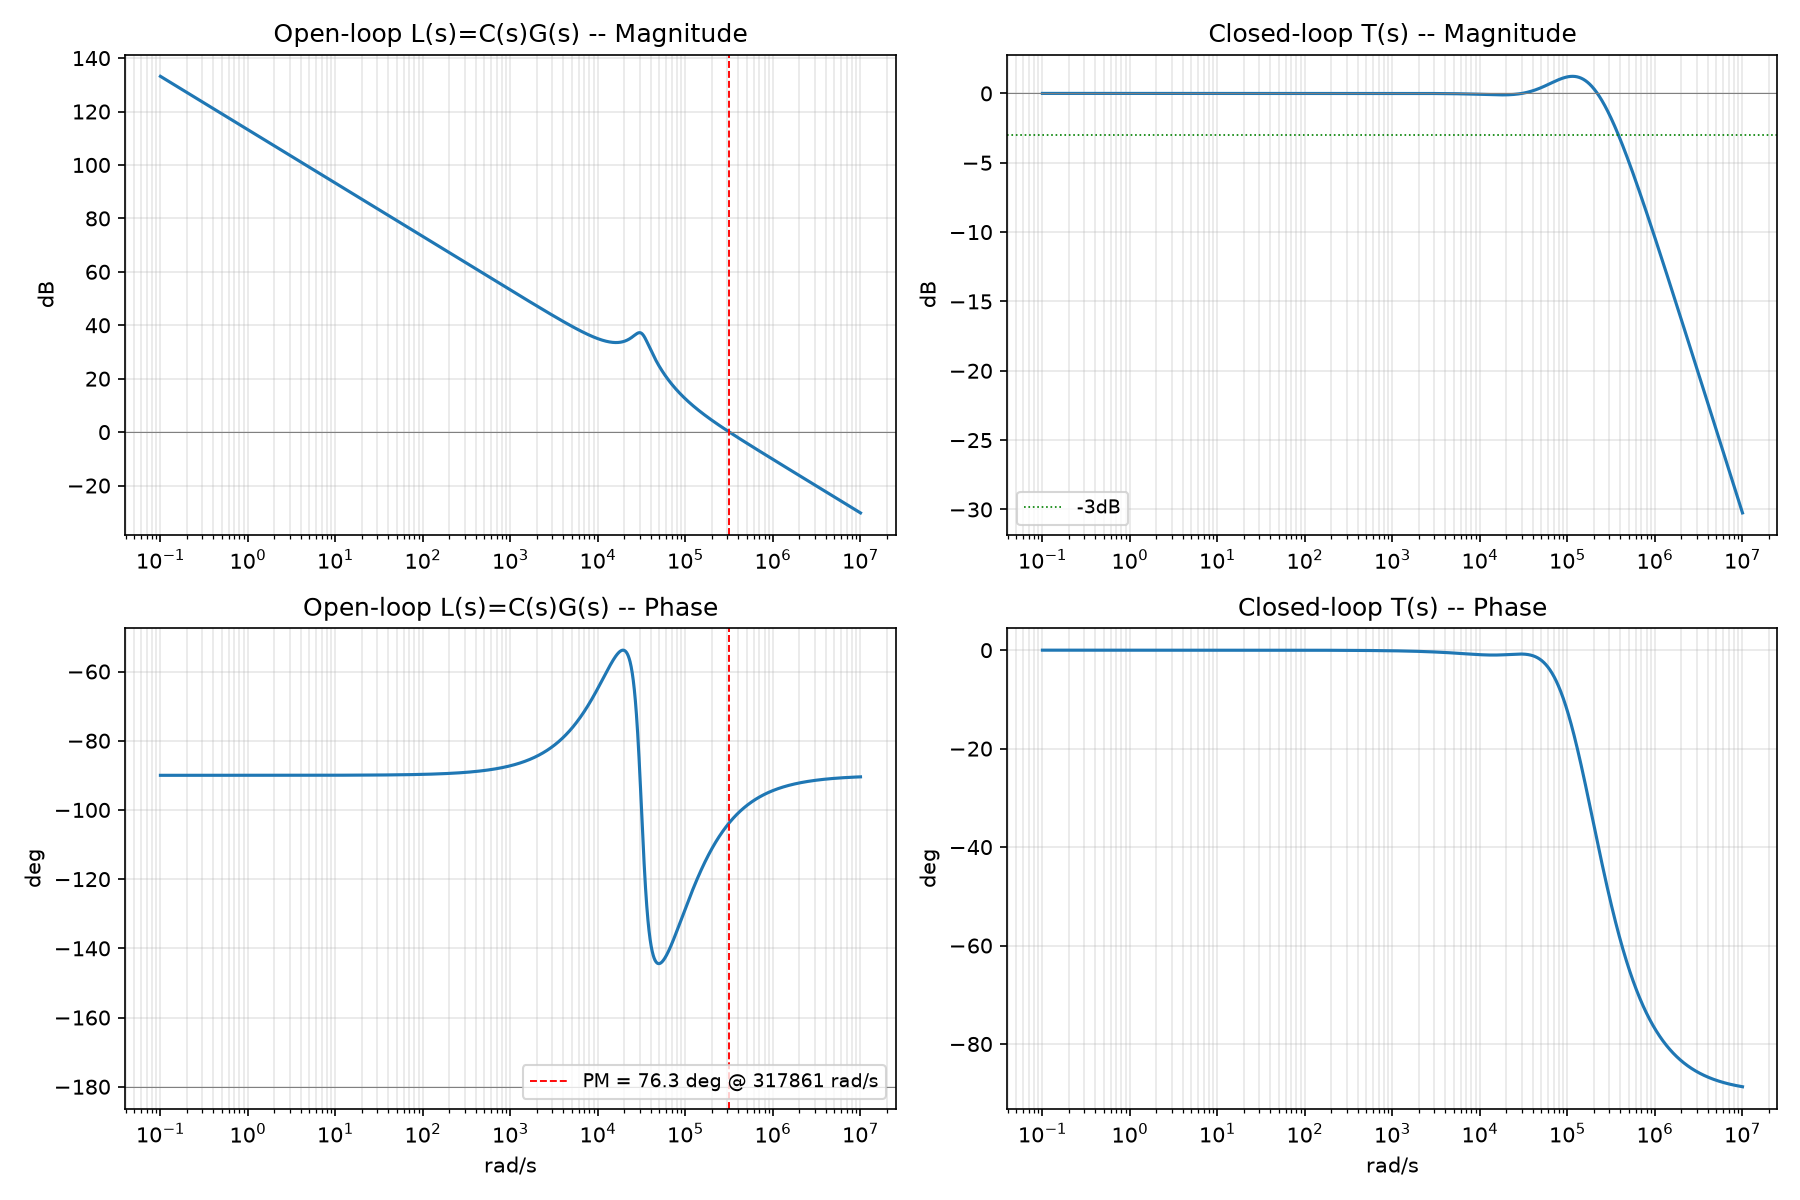
\includegraphics[width=0.95\textwidth]{figures/bode_plot.png}
\caption{Open-loop $L(s)$ magnitude/phase (left) and closed-loop $T(s)$ magnitude/phase (right), computed
from the actual plant and controller transfer functions.}
\label{fig:bode}
\end{figure}

The single gain crossover ($|L(j\omega)|=\SI{0}{\decibel}$) occurs at $\omega_c\approx\SI{317861}{rad/s}$,
with phase margin $\mathrm{PM}\approx76.3^\circ$ -- a healthy margin (above the usual 45--60$^\circ$
design target). The open-loop phase never reaches $-180^\circ$ across the swept range
($10^{-1}$ to $10^{7}$~rad/s), so there is no classical gain-margin crossover to report; this is
consistent with the all-real-closed-loop-pole design (Section~4.3), which by construction has no
oscillatory mode. The closed-loop magnitude shows a small ($\approx$\SI{1}{\decibel}) peak near
$1$--$2\times10^5$~rad/s before rolling off, and stays flat near \SI{0}{\decibel} well below that --
consistent with good reference tracking without excessive resonant peaking.

\begin{pending}
Whether the derivative term is implemented as a full analog PID or simplified to PI-only for noise
immunity (Section~5) -- if $K_d$ is implemented, it must be through the \emph{filtered/band-limited
derivative} discussed in Section~5, not an ideal differentiator, since an ideal derivative would amplify
any high-frequency noise on the feedback signal.
\end{pending}

% ======================================================================
\section{Op-Amp Compensator Circuit}

\subsection{Topology: five op-amp stages}

The parallel PID (Section~4.1) is realized as five op-amp stages: a difference amplifier computing the
error, three parallel branches (P, I, filtered-D) acting on that error, and a summing amplifier
recombining them.

\subsection*{General basis: the inverting amplifier}

Every branch below is a special case of the same ideal-op-amp result (virtual ground at the inverting
input + KCL at that node, standard inverting-amplifier analysis):

\begin{tcolorbox}[colback=blue!5,colframe=blue!40!black,arc=1mm]
\begin{equation}
\frac{V_{out}}{V_{in}} = -\frac{Z_f}{Z_{in}}
\end{equation}
\end{tcolorbox}

where $Z_{in}$ and $Z_f$ are the input and feedback impedances. Only the choice of components placed in
those two positions changes between branches:

\begin{enumerate}[nosep]
    \item \textbf{Difference amplifier:} computes $e(t)=V_{ref}-V_C$ from the reference and the plant's
    feedback signal (standard four-resistor differential amplifier, not derived from the formula above).
    \item \textbf{Proportional branch:} $Z_{in}=R_p$, $Z_f=R_{fp}$ (both plain resistors):
    \begin{equation}
    \frac{V_{out,P}}{e} = -\frac{R_{fp}}{R_p} \;\Rightarrow\; K_p=\frac{R_{fp}}{R_p}
    \end{equation}
    \item \textbf{Integral branch:} $Z_{in}=R_i$, $Z_f=\frac{1}{sC_i}$ (a capacitor's impedance replaces
    the feedback resistor):
    \begin{equation}
    \frac{V_{out,I}}{e} = -\frac{1/(sC_i)}{R_i} = -\frac{1}{sR_iC_i} \;\Rightarrow\; K_i=\frac{1}{R_iC_i}
    \end{equation}
    (division by $s$ in Laplace corresponds to integration in time, hence $V_{out,I}=-\frac{1}{R_iC_i}\int e\,dt$).
    \item \textbf{Filtered-derivative branch:} $Z_{in}=R_1+\frac{1}{sC_d}$ (a resistor in series with a
    capacitor -- series impedances add), $Z_f=R_{fd}$:
    \begin{equation}
    \frac{V_{out,D}}{e} = -\frac{R_{fd}}{R_1+\frac{1}{sC_d}} = \frac{-R_{fd}C_d\,s}{1+sR_1C_d}
    \end{equation}
    giving $K_d=R_{fd}C_d$ at low frequency, capped at $-R_{fd}/R_1$ above the corner frequency
    $f_{pole}=1/(2\pi R_1 C_d)$ -- this avoids amplifying high-frequency noise, unlike an ideal
    differentiator ($R_1=0$, bare capacitor), whose gain grows unboundedly with frequency.
    \item \textbf{Summing amplifier:} recombines the three branch outputs (each through an equal input
    resistor $R_s$, feedback $R_{fs}$) into $u(t)=K_pe+K_i\int e\,dt+K_d\frac{de}{dt}$, which drives the
    plant.
\end{enumerate}

\subsection{Component values}

Design choice: $R_p=R_i=R_{fd}=\SI{10}{\kilo\ohm}$ (a common reference value across stages -- reduces
distinct BOM part count, and $\SI{10}{\kilo\ohm}$ is a practical general-purpose value for op-amp input
resistors: high enough to not load the driving stage's output, low enough that op-amp input bias current
and noise stay negligible). The remaining component in each branch follows directly:

\begin{align}
R_{fp} &= K_p R_p = 27.87\times10{,}000 \approx \SI{278.7}{\kilo\ohm} \\
C_i &= \frac{1}{K_i R_i} = \frac{1}{455{,}905\times10{,}000} \approx \SI{219.3}{\pico\farad} \\
C_d &= \frac{K_d}{R_{fd}} = \frac{3.114\times10^{-4}}{10{,}000} \approx \SI{31.14}{\nano\farad}
\end{align}

\subsection*{Filtered-derivative corner frequency and $R_1$}

The corner (pole) frequency of the filtered-derivative branch, in rad/s, is $\omega_{pole}=1/(R_1C_d)$
(the pole of $1+sR_1C_d$). Below $\omega_{pole}$ the branch acts as a real differentiator (gain growing
with frequency, providing the intended phase lead within the control loop's bandwidth); above it, the
gain flattens at a fixed value $R_{fd}/R_1$ instead of continuing to grow, which is what prevents
high-frequency noise from being amplified without bound. Criterion: place $\omega_{pole}$ comfortably
above the gain crossover frequency ($\approx\SI{317861}{rad/s}$, Section~4.5) so the entire
control-relevant frequency range sees real derivative action, with the noise-limiting flattening only
taking effect well beyond it. Choosing $\omega_{pole}\approx\SI{2e6}{rad/s}$ ($\approx6.3\times$ the gain
crossover):

\begin{equation}
R_1 = \frac{1}{\omega_{pole}C_d} = \frac{1}{(2\times10^6)(31.14\times10^{-9})} \approx \boxed{\SI{16.06}{\ohm}}
\end{equation}

\subsection*{Summing and difference amplifiers}

\textbf{Summing amplifier:} each branch (P, I, D) already carries its own gain ($K_p$, $K_i$, $K_d$)
from its own stage, so the summer only needs to add the three signals with unity gain, which requires
equal input and feedback resistors: $R_s=R_{fs}=\SI{10}{\kilo\ohm}$ (consistent with the rest of the
design).

\textbf{Difference amplifier:} the standard 4-resistor differential amplifier gives unity gain
($e=V_{ref}-V_C$ exactly, no scaling) when all four resistors are equal: all four set to
$\SI{10}{\kilo\ohm}$.

\subsection{Full schematic, by stage}

Shown one stage at a time (clearer to build from than a single combined diagram). Signal flow:
$V_{ref}$ and $V_C$ (feedback) $\to$ difference amp $\to e(t) \to$ P/I/D branches in parallel
$\to$ summing amp $\to u(t) \to$ plant (series RLC, Section~3) $\to V_C$, closing the loop.

\begin{figure}[H]
\centering
\begin{circuitikz}[scale=1.0, transform shape]
\draw (4.0,1.5) node[op amp](A1){};
\draw (0,1.5) node[anchor=east]{$V_C$ (feedback)} to[R=$10k$] (4.0,1.5);
\coordinate (pnode) at (2.5,0.3);
\draw (0,0.3) node[anchor=east]{$V_{ref}$} to[R=$10k$] (pnode) -- (A1.+);
\draw (pnode) to[R=$10k$] ++(0,-1.0) node[ground]{};
\draw (A1.-) ++(0,1.1) to[R=$10k$] ++(2.4,0) |- (A1.out);
\draw (A1.out) -- ++(1.2,0) node[anchor=west]{$e(t) = V_{ref}-V_C$};
\end{circuitikz}
\caption{Stage 1 -- difference amplifier. All four resistors $10k\Omega$. $V_{ref}\to(+)$,
$V_C\to(-)$, giving $e=V_{ref}-V_C$ (not the reverse).}
\end{figure}

\begin{figure}[H]
\centering
\begin{circuitikz}[scale=1.0, transform shape]
\draw (0,1.5) node[anchor=east]{$e(t)$} to[R=$R_p{=}10k$] (2.5,1.5) -- (2.8,1.0) node[op amp](A2){};
\draw (A2.+) -- ++(-0.9,0) node[ground]{};
\draw (A2.-) ++(0,1.0) to[R=$R_{fp}\approx278.7k$] ++(2.4,0) |- (A2.out);
\draw (A2.out) -- ++(1.2,0) node[anchor=west]{$-K_p\,e$};
\end{circuitikz}
\caption{Stage 2 -- P branch. Simple inverting amplifier. $K_p=R_{fp}/R_p\approx27.87$.}
\end{figure}

\begin{figure}[H]
\centering
\begin{circuitikz}[scale=1.0, transform shape]
\draw (0,1.5) node[anchor=east]{$e(t)$} to[R=$R_i{=}10k$] (2.5,1.5) -- (2.8,1.0) node[op amp](A3){};
\draw (A3.+) -- ++(-0.9,0) node[ground]{};
\draw (A3.-) ++(0,1.0) to[C=$C_i\approx219.3p$] ++(2.4,0) |- (A3.out);
\draw (A3.out) -- ++(1.2,0) node[anchor=west]{$-K_i\!\int e\,dt$};
\end{circuitikz}
\caption{Stage 3 -- I branch. Same as P, but a \textbf{capacitor} instead of a resistor in the
feedback path -- that is what makes it an integrator. $K_i=1/(R_iC_i)\approx455{,}905$.}
\end{figure}

\begin{figure}[H]
\centering
\begin{circuitikz}[scale=1.0, transform shape]
\draw (0,1.5) node[anchor=east]{$e(t)$} to[R=$R_1\approx16.06\Omega$] (2.7,1.5) to[C=$C_d\approx31.14n$] (5.2,1.5) -- (5.5,1.0) node[op amp](A4){};
\draw (A4.+) -- ++(-0.9,0) node[ground]{};
\draw (A4.-) ++(0,1.0) to[R=$R_{fd}{=}10k$] ++(2.4,0) |- (A4.out);
\draw (A4.out) -- ++(1.2,0) node[anchor=west]{$-K_d\dot{e}$ (filtered)};
\end{circuitikz}
\caption{Stage 4 -- filtered D branch. The input is $R_1$ in series with $C_d$ (not a bare
capacitor -- that would be an ideal, noise-amplifying differentiator). This caps the gain above
$f_{pole}=1/(2\pi R_1 C_d)$.}
\end{figure}

\begin{figure}[H]
\centering
\begin{circuitikz}[scale=1.0, transform shape]
\draw (0,3.0) node[anchor=east]{$-K_pe$} to[R=$R_s{=}10k$] (2.8,3.0);
\draw (0,1.5) node[anchor=east]{$-K_i\!\int e\,dt$} to[R=$R_s{=}10k$] (2.8,1.5);
\draw (0,0.0) node[anchor=east]{$-K_d\dot{e}$} to[R=$R_s{=}10k$] (2.8,0.0);
\draw (2.8,3.0) -- (2.8,0.0);
\draw (4.6,1.5) node[op amp](A5){};
\draw (2.8,1.5) -- (A5.-);
\draw (A5.+) -- ++(-0.9,0) node[ground]{};
\draw (A5.-) ++(0,1.0) to[R=$R_{fs}{=}10k$] ++(2.4,0) |- (A5.out);
\draw (A5.out) -- ++(1.2,0) node[anchor=west]{$u(t)$};
\end{circuitikz}
\caption{Stage 5 -- summing amplifier. The three inputs already carry their own gain; the summer
just adds them (unity gain, $R_s=R_{fs}$). Its output $u(t)$ drives the plant (series RLC,
Section~3) in place of the step source used for the open-loop test.}
\label{fig:full-schematic}
\end{figure}

\textbf{Simulated.} Built exactly as above in LTspice and run closed-loop, with $V_{ref}$ as a
\texttt{PULSE(0 1 0 10u 10u 10 10)} source (same 1V step as the open-loop test, 10\textmu s rise time
-- see Section~6.1 for why an idealized 1ns rise time was rejected). Op-amps modeled with LTspice's
\texttt{opamp} subcircuit (\texttt{.lib opamp.sub}), $A_{ol}=100k$, GBW raised above the library default
of 10MHz to keep each stage's own bandwidth well clear of the loop dynamics (Section~6.2).

\subsection*{Possible failure point: parasitic capacitance on $C_i$}

$C_i\approx\SI{219.3}{\pico\farad}$ is small enough that breadboard/PCB stray capacitance (typically
\SIrange{1}{5}{\pico\farad} for a breadboard node) is a non-negligible fraction of it ($\approx$1--2\%).
If the built integrator's measured $K_i$ deviates noticeably from the calculated \num{455905}, this
parasitic pickup -- not necessarily a design or calculation error -- should be the first thing checked,
before re-deriving the gains. Mitigation if it proves significant: reduce $R_i$ (increasing $C_i$
proportionally to keep the same $K_i=1/(R_iC_i)$, at the cost of loading the source driving this branch
more).

% ======================================================================
\section{SPICE Simulation (LTspice)}

\subsection{Open-loop}

\textbf{Done} -- see Section~3.1 (52.68\% simulated vs.\ 52.7\% predicted, extracted numerically from
the \texttt{.raw} file).

\subsection{Closed-loop: debugging}

Two real issues were hit and resolved before a valid closed-loop result was obtained -- documented
here since both are genuine, non-obvious LTspice pitfalls, not modeling mistakes in the design itself.

\textbf{1. Undefined subcircuit.} The first run failed with \texttt{"This sub-circuit name is not
defined"} for all five op-amps. Cause: LTspice's basic \texttt{opamp} symbol is not auto-linked to its
model -- its own description text says \textit{"You must .lib opamp.sub"}. Fix: added
\texttt{.lib opamp.sub} as a schematic text directive.

\textbf{2. Numeric overflow ($\sim 4\times10^{38}$V).} With the missing-library issue fixed, the first
successful netlist run produced an output that grew to floating-point overflow -- the signature of
positive feedback / loop instability, not a slowly-diverging but otherwise sane result. The generated
netlist was checked node-by-node against the intended design (Sections~4.4--5) and matched exactly --
no wiring error. The actual cause: LTspice's \texttt{opamp} model is not truly ideal even at its default
settings -- it carries a finite gain-bandwidth product, \texttt{GBW=10Meg} (10MHz), by default. With
$K_p\approx27.87$, the P-branch's own bandwidth is only $\text{GBW}/K_p\approx\SI{358}{\kilo\hertz}$,
close enough to the design's own dynamics (D-branch corner $\approx\SI{318}{\kilo\hertz}$, Section~5)
that the cumulative phase lag from five cascaded finite-bandwidth stages ate into the phase margin
(Section~4.5) enough to destabilize the loop. Fix: raised \texttt{GBW} well above this design's
frequencies of interest, confirming the diagnosis (the instability disappeared).

\subsection{Closed-loop: result}

With both issues resolved, the closed-loop step response was obtained:

\begin{center}
\begin{tabular}{@{}ll@{}}
\toprule
Peak $V_C$ & \SI{1.11539}{\volt}, at $t=\SI{17.37}{\micro\second}$ \\
Final (settled) $V_C$ & \SI{0.99999}{\volt} \\
Overshoot & $(1.11539-1)/1\times100 = \boxed{11.54\%}$ \\
Settled within $\pm2\%$ & by $t\approx\SI{31.5}{\micro\second}$ \\
\bottomrule
\end{tabular}
\end{center}

This is a large improvement over the \SI{52.68}{\percent} open-loop result, but not the
\SI{0}{\percent} predicted by the all-real-closed-loop-pole design criterion of Section~4.3. Two
hypotheses were tested:

\textbf{Hypothesis A (rejected): step edge speed exciting the D-branch.} The reference step's rise time
was changed from an idealized 1ns to a more realistic \SI{10}{\micro\second} (10,000$\times$ slower).
Overshoot only dropped from \SI{13.26}{\percent} to \SI{11.54}{\percent}, and the peak timing barely
moved (\SI{11.3}{}$\to$\SI{17.4}{\micro\second}) -- far too small a change for edge speed to be the
dominant cause. Rejected by this data.

\textbf{Hypothesis B (supported): closed-loop zero near the dominant pole.} The all-real-pole design
criterion (Section~4.3) is sufficient to rule out any oscillatory \emph{pole}, but the closed-loop
transfer function also has \emph{zeros}, from the PID's own numerator ($K_ds^2+K_ps+K_i=0$) -- not
accounted for in the original pole-placement criterion. Solving for the actual zeros with the derived
gains:
\begin{equation}
K_ds^2+K_ps+K_i=0 \;\Rightarrow\; z_{1,2} \approx -21{,}524 \text{ and } -67{,}979 \text{ rad/s}
\end{equation}
$z_1\approx-21{,}524$ rad/s sits almost on top of the dominant pole ($p_1=-20{,}000$ rad/s, Section~4.3)
-- a near pole-zero cancellation. When a zero nearly cancels the dominant (slowest) pole, the visible
response is no longer dominated by that $\sim\SI{200}{\micro\second}$ time constant -- it is dominated
by the remaining, much faster dynamics (the non-dominant poles at $-150{,}000$ rad/s, $\tau\approx\SI{6.7}{\micro\second}$,
and the second zero at $z_2\approx-67{,}979$ rad/s, $\tau\approx\SI{14.7}{\micro\second}$), which matches
the observed \SI{11}{}--\SI{31}{\micro\second} transient far better than the design's nominal
\SI{200}{\micro\second} target. A real pole-zero pair (both on the negative real axis, not complex) can
still produce step-response overshoot when imperfectly cancelled -- a real, documented limitation of the
pole-placement method used, not a simulation artifact.

\textbf{Decision:} the \SI{11.54}{\percent} result is accepted as final for this project phase, given
the trade-off explored in Section~\ref{sec:pz-explore}.

\subsection{Pole placement revisited: why not just re-tune?}
\label{sec:pz-explore}

A systematic search (varying the dominant pole magnitude and its separation ratio from the non-dominant
poles, and separately trying a complex dominant pole pair with $\zeta=0.7$) found that a zero landing
near the dominant pole is a persistent, structural feature of this plant-plus-PID combination, not a
poor choice of one specific pole triple: every fast/practical candidate tested still put a zero within
\SI{4}{}--\SI{25}{\percent} of the dominant pole. Materially improving that separation required slowing
the dominant pole down (e.g.\ to $\sim$\SI{5000}{rad/s}, $\tau\approx\SI{800}{\micro\second}$) -- slower
than the \emph{open-loop} response itself, defeating the purpose of adding control. This trade-off
(speed vs.\ overshoot, given this specific plant) is the actual reason \SI{11.54}{\percent} was accepted
rather than chased further.

% ======================================================================
\section{Conclusions}

\begin{enumerate}
    \item The open-loop plant matched its analytical prediction almost exactly (\SI{52.68}{\percent}
    simulated vs.\ \SI{52.7}{\percent} calculated overshoot), validating both the transfer-function
    derivation (Section~3) and its SPICE implementation before any control was added.
    \item A parallel PID, designed by direct algebraic pole placement (3 free gains for a 3rd-order
    closed-loop characteristic equation, Section~4), reduced the overshoot from \SI{52.68}{\percent}
    (open-loop) to \SI{11.54}{\percent} (closed-loop) -- a large, real improvement, though not the
    \SI{0}{\percent} the all-real-pole criterion predicted.
    \item \textbf{Key limitation found:} an all-real-pole closed-loop design guarantees no oscillatory
    \emph{pole}, but does not by itself guarantee zero step-response overshoot, because the PID
    contributes its own \emph{zeros} to the closed-loop transfer function. For this plant, a zero
    consistently lands near the dominant pole across a wide range of pole choices (Section~6.5) -- a
    structural property of this specific plant-plus-PID combination, confirmed by systematically
    searching the design space, not a one-off tuning mistake.
    \item Two real LTspice pitfalls were hit and resolved during closed-loop debugging: the generic
    \texttt{opamp} symbol requires a manual \texttt{.lib opamp.sub} directive, and that same symbol's
    default gain-bandwidth product (10MHz) was not fast enough for this specific design (five cascaded
    stages, $K_p\approx27.87$) without destabilizing the loop -- both documented in Section~6.2 so they
    are not rediscovered from scratch on the next project (the PID-controlled buck).
    \item The op-amp compensator was fully specified with real, standard component values
    ($R_p=R_i=R_{fd}=R_s=R_{fs}=\SI{10}{\kilo\ohm}$, $R_{fp}\approx\SI{278.7}{\kilo\ohm}$,
    $C_i\approx\SI{219.3}{\pico\farad}$, $R_1\approx\SI{16.06}{\ohm}$, $C_d\approx\SI{31.14}{\nano\farad}$,
    Section~5), and the filtered-derivative design (a lead network, not an ideal differentiator) was
    carried through consistently to avoid amplifying switching/measurement noise.
    \item \SI{11.54}{\percent} overshoot, well-characterized and understood, is accepted as the final
    result for this project phase rather than chased further, given the documented speed-vs-overshoot
    trade-off (Section~6.5).
\end{enumerate}

\end{document}
